\section{Monitoring}

To efficiently manage the service, a solid monitoring infrastructure is required. The new monitoring infrastructure of CASTOR is mainly based on log message analysis. This was made possible by the improvements of the different components of the system, so that they can report every action to their respective log files. Subsequently, a transport layer was deployed in order to ship these messages to different systems: the {\it LogViewer} to browse in real time the log records, the {\it Metric Analysis Engine} and the {\it Cockpit} to compute a set of metrics in real time over the flow of log messages, and finally an Hadoop FS is used to archive and enable data mining.


\subsection{Transport}

Every CASTOR component produces its own log files. These files are distributed (not evenly) in all the machines that are part of a CASTOR cluster. The first challenge of the new monitoring infrastructure was to transport these log files:
\begin{itemize}
\item efficiently, to be able to follow the high production rate and minimize the footprint and the extra resources needed (operation and hardware)
\item quickly, to enable real-time analysis
\item reliably, to prevent the loss of any message
\item modularly, to be able to easily replace any block of the transport sub-system in the future
\end{itemize}
These requirements were fulfilled with a modular architecture proposed by the team maintaining the messaging brokers of the CERN IT department, as can be seen in Figure \ref{fig:arch}.
A generic producer, named \texttt{simple-log-producer}, takes care of reading the different log files as they are written, similarly to the \texttt{tail} Unix command. Each line is considered as a unique and independent log record, which is then sent to the transport layer brokers using the STOMP protocol.
The multiple Apache ActiveMQ brokers deployed in the IT department are running behind a DNS alias, to bring high availability and load balancing. Here we \textit{produce to any, consume from all}. So the producers just need to send their messages to any broker behind the alias. However, the consumers need to consume from all the brokers. This is achieved by using a dynamic configuration file, which is updated each time a broker appears or disappears in the alias.

\begin{figure}[h]
\begin{center}
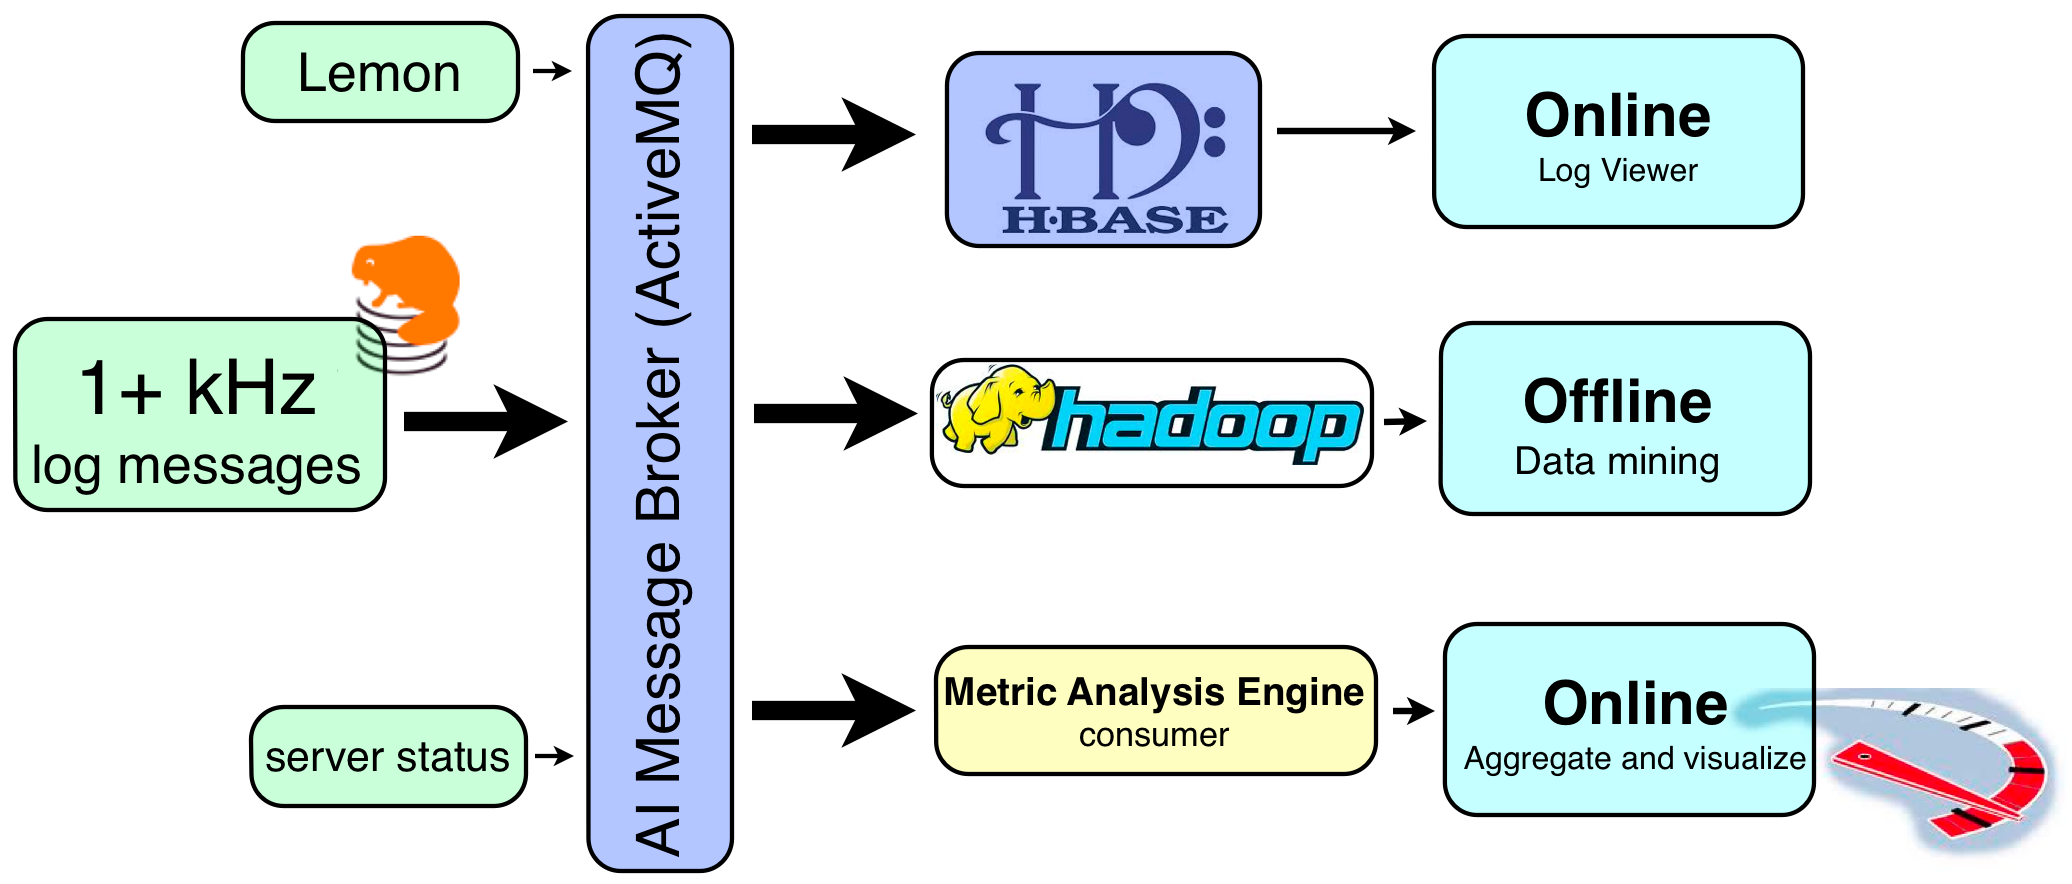
\includegraphics[width=32pc]{monitoring_architecture.png}
\caption{\label{fig:arch}The Monitoring architecture, with the IT Agile Infrastructure Message Broker and the components developed around it.
Among the inputs, Lemon [LHC Era Monitoring] provides basic hardware monitoring, and the CASTOR aggregated logs represent the bulk of the load at over 1 kHz rate.}
\end{center}
\end{figure}


\subsection{The LogViewer}

A tool to browse the log records is crucial for the developers and the operators of the service in order to debug and investigate operational issues. To meet this need, a simple consumer was developed. Its role is to insert the records in a column oriented database, \textit{Apache HBase}.
To determine the best schema, the query patterns were carefully analysed. It appeared that the logs needed to be queried by only three keys:
\begin{itemize}
\item file ID, to look into whole history of a file
\item request ID, to look into the history of a request
\item tape ID, to study the whole life of a tape
\end{itemize}
Therefore, after testing, it was decided to use these three keys as a HBase object key, and store the entire raw messages in the columns. Hence it is trivial to retrieve the entire set of required messages with a single query by object key. In a real-life example, the system returned nearly 180,000 records in 16.7 seconds, which compares well with traditional SQL-based technologies.

A Django web application was developed, in order to easily browse the HBase database: it allows querying by any of the three keys, and displays the list of corresponding log messages.


\subsection{The Metric Analysis Engine and the Cockpit}

The Metric Analysis Engine (MAE) is a framework designed to compute a set of metrics from the flow of messages. The input is a Python dictionary, and the output is another Python dictionary with computed values, aggregated as defined in a metric definition file. The following code describes a metric which counts the number of error message, over a 60 second sliding window using 3 bins. The results are also broken down by instance and daemon.
\scriptsize
\begin{verbatim}
<metric>
    name: Errors
    window: 60
    conditions: LVL == "Error"
    groupbykeys: INSTANCE, DAEMON
    data: Counter(COUNT)
    nbins: 3
</metric>
\end{verbatim}
\normalsize

A consumer for the transport layer was developed using the MAE framework. This component has two other roles: feeding a Django web application (the Cockpit) with the computed metric values, and making the computed metric values available via an RPC interface.

The Cockpit is capable of plotting and displaying the different metrics computed by the MAE in time series charts or histograms, as shown in Figure \ref{fig:scr}. It receives the metrics data via a REST (Representational State Transfer) interface, and stores the samples in a MySQL database.


\subsection{The HDFS Archive}

The last consumer component is responsible for archiving the log messages in the Hadoop Distributed File System (HDFS). The two main goals of this archive are the long term storage of the logs in an independent file system, and the ability to execute data mining analyses by means of the Hadoop \textit{MapReduce} framework.

Log messages are stored in this archive using the following hierarchy: the first level is the cluster name, e.g. \texttt{castorpublic}, the second level is the node type (head node or storage node), and the third level is the date. The consumer processes aggregate the messages before sending them to HDFS. Afterwards, MapReduce jobs are run to aggregate and merge the small files into larger chunks, more suitable for storing in HDFS.

This archive enables operators to run specialized data-mining analysis by writing simple MapReduce jobs to be run on Hadoop, thus exploiting the parallelism and data locality offered by the system. For instance, a typical activity is to run a trend analysis on a particular log message. On a traditional file-based store this would require executing multiple \texttt{grep}-like operations on several files scattered in different machines, and then aggregating the results by hand. The Hadoop streaming interface allows writing simple scripts for the Map and Reduce phases, and the interface takes care of running jobs to collect all aggregated results in one go at the end of their execution.

\begin{figure}[h]
\begin{center}
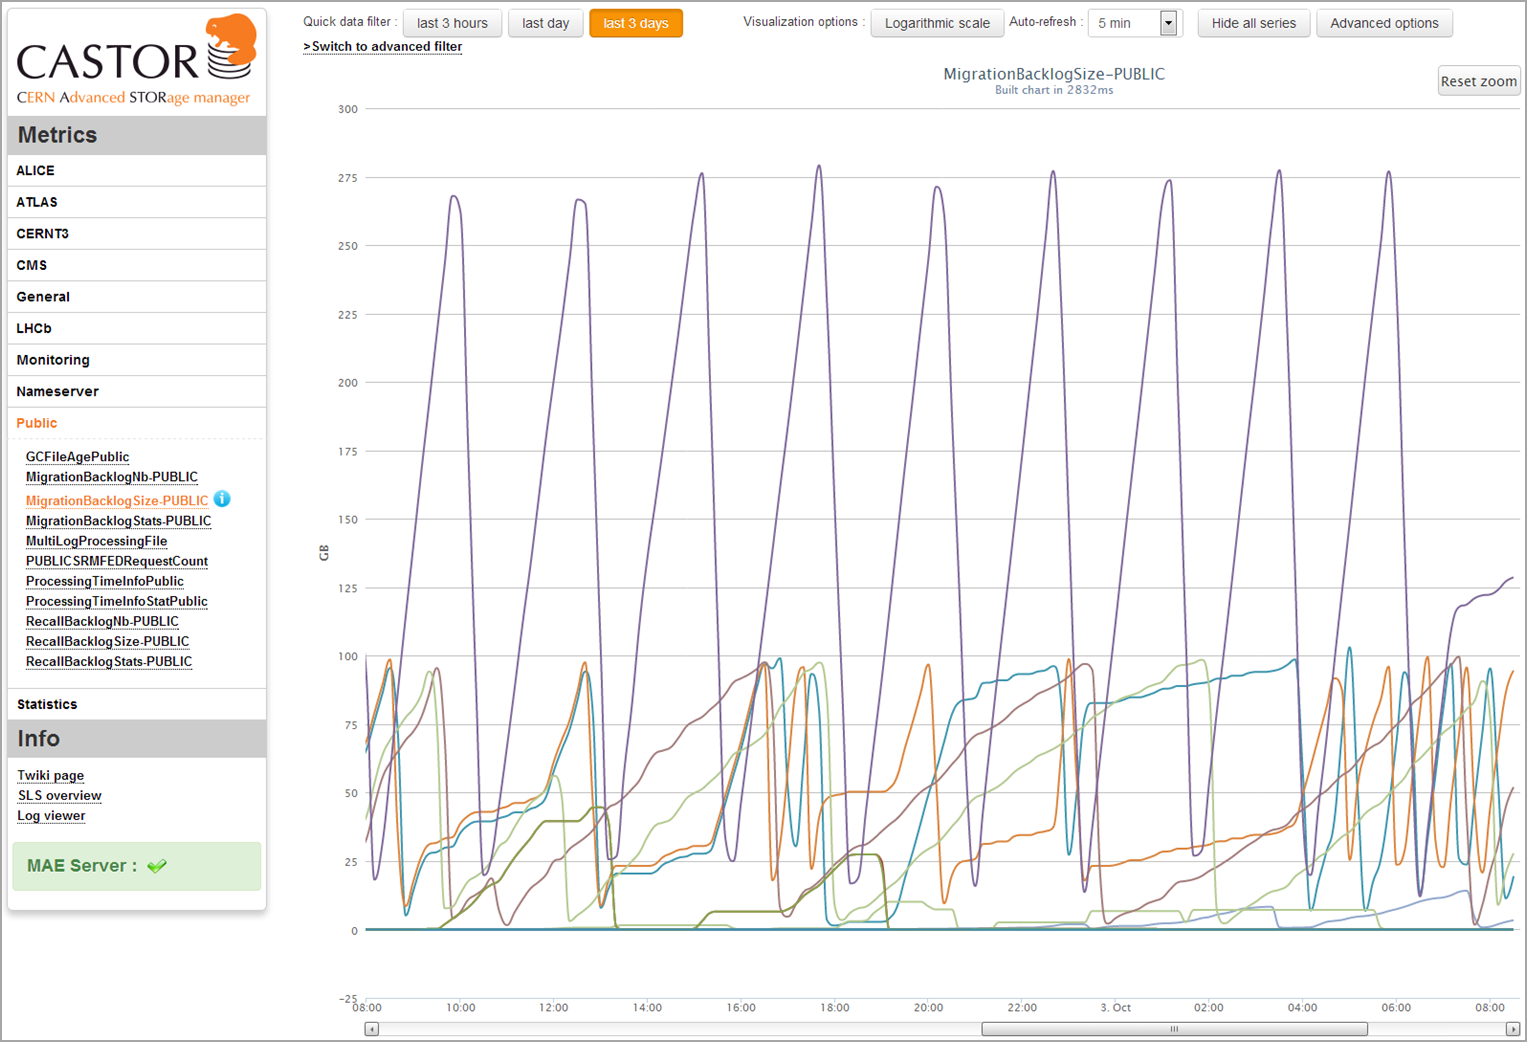
\includegraphics[width=36pc]{cockpit_screenshot.png}
\caption{\label{fig:scr}An illustrative screenshot of the Cockpit interface, showing for instance the migration-to-tape queue during 24 hours for the \texttt{castorpublic} cluster.}
\end{center}
\end{figure}
